\begin{table*}[htbp]
\centering
\caption{Deep Learning Frameworks}
\label{table_framework}
\begin{small}
\begin{tabular}{l|l|l|l|l|l}
\hline\hline
  Framework & Developer  & Single GPU & Multi-GPUs        & Operating & User \\
            &            &            & (parallelism)     & system    & interface \\
\hline
Caffe      & BVLC & Supported & Data           & Linux & protobuf, Python, MATLAB \\
CNTK       & Microsoft   & Supported & Data           & Windows, Linux & BrainScript, C++, C\#\\
TensorFlow & Google      & Supported & Data, Model    & Linux & Python, C++\\
Theano     & Theano Development Team  & Supported & None  & Linux & Python \\
Torch      &    & Supported & Data, Model  & Linux & LuaJIT \\  
\hline      
\end{tabular}
\end{small}
\end{table*}

\section{Background and Related work}
In this section, we briefly describe the five major deep learning frameworks and a typical organization of CNNs. We also introduces some related work about comparative studies of deep learning frameworks.

\subsection{Deep Learning Frameworks}
There are five major deep learning frameworks that are frequently used by users to build deep learning models: Caffe\cite{jia2014caffe}, CNTK (Computational Network Toolkit)\cite{cntk}, TensorFlow\cite{tensorflow2015-whitepaper}, Theano\cite{DBLP:journals/corr/Al-RfouAAa16}, and Torch\cite{torch}. Table~\ref{table_framework} summarizes these five major deep learning frameworks. We will describe the data parallelism and model parallelism later in this section. \Comment{$<$==== complete the table ===}

Visual recognition challenge winners are usually implemented with Caffe\cite{ILSVRC15, RCNN, vgg}. However, the flexibility of Caffe is somehow limited. Introducing a new feature to a layer requires re-building the entire source code. TensorFlow was publicly introduced in 2015 and is now the most popular machine learning framework in GitHub\cite{github}. Theano one of the earliest deep learning frameworks. Pylearn2\cite{pylearn2}, Keras\cite{keras}, and Lasagne\cite{lasagne} are popular DNN frameworks that use Theano as their backend. However, The Multi-GPU support of Theano is still in an experimental stage. Torch is a scientific computing framework based on LuaJIT\cite{torch}. It is also one of the earliest DNN frameworks. Nvidia's self-driving car project\cite{nvdave} and Deepmind's Deep Q Learning model\cite{mnih2015humanlevel} were built on top of it.

\subsection{Convolutions}
A convolution is an operation between two functions. It creates a new function defined as an integration of translated pointwise multiplication of given two functions:
\begin{equation}
\left ( f * g \right )(t) = \int f(x)g(t-x)dx = \int f(t-x)g(x)dx
\label{def_convolution}
\end{equation}
The convolution operation is commutative and its value shows the degree of similarity between the two functions $f$ and $g$. Convolutions can also be naturally defined for discrete values. We can define the convolution of two finite sequences $f[i]$ and $g[i]$ as follows:
\begin{equation}
\label{def_discrete}
\left ( f * g \right )[n] = \sum_{1}^{M} f[n + m]g[m]
\end{equation}
The convolution operation can be extended to multiple dimensions. A two-dimensional (2D) convolution between filter (a.k.a. a kernel) $F[r][s] \; (0 \leq r \leq R, 0 \leq s \leq S)$ and data $D[h][w] \; (0 \leq h \leq H, 0 \leq w \leq W)$ can be described with the following equation:
\begin{equation}
\label{def_2d}
\left ( D * F \right )[h][w] = \sum_{1}^{R}\sum_{1}^{S} D[h + r][w + s] F[r][s]
\label{2d-conv}
\end{equation}

\begin{figure}[htbp]
  \centering
  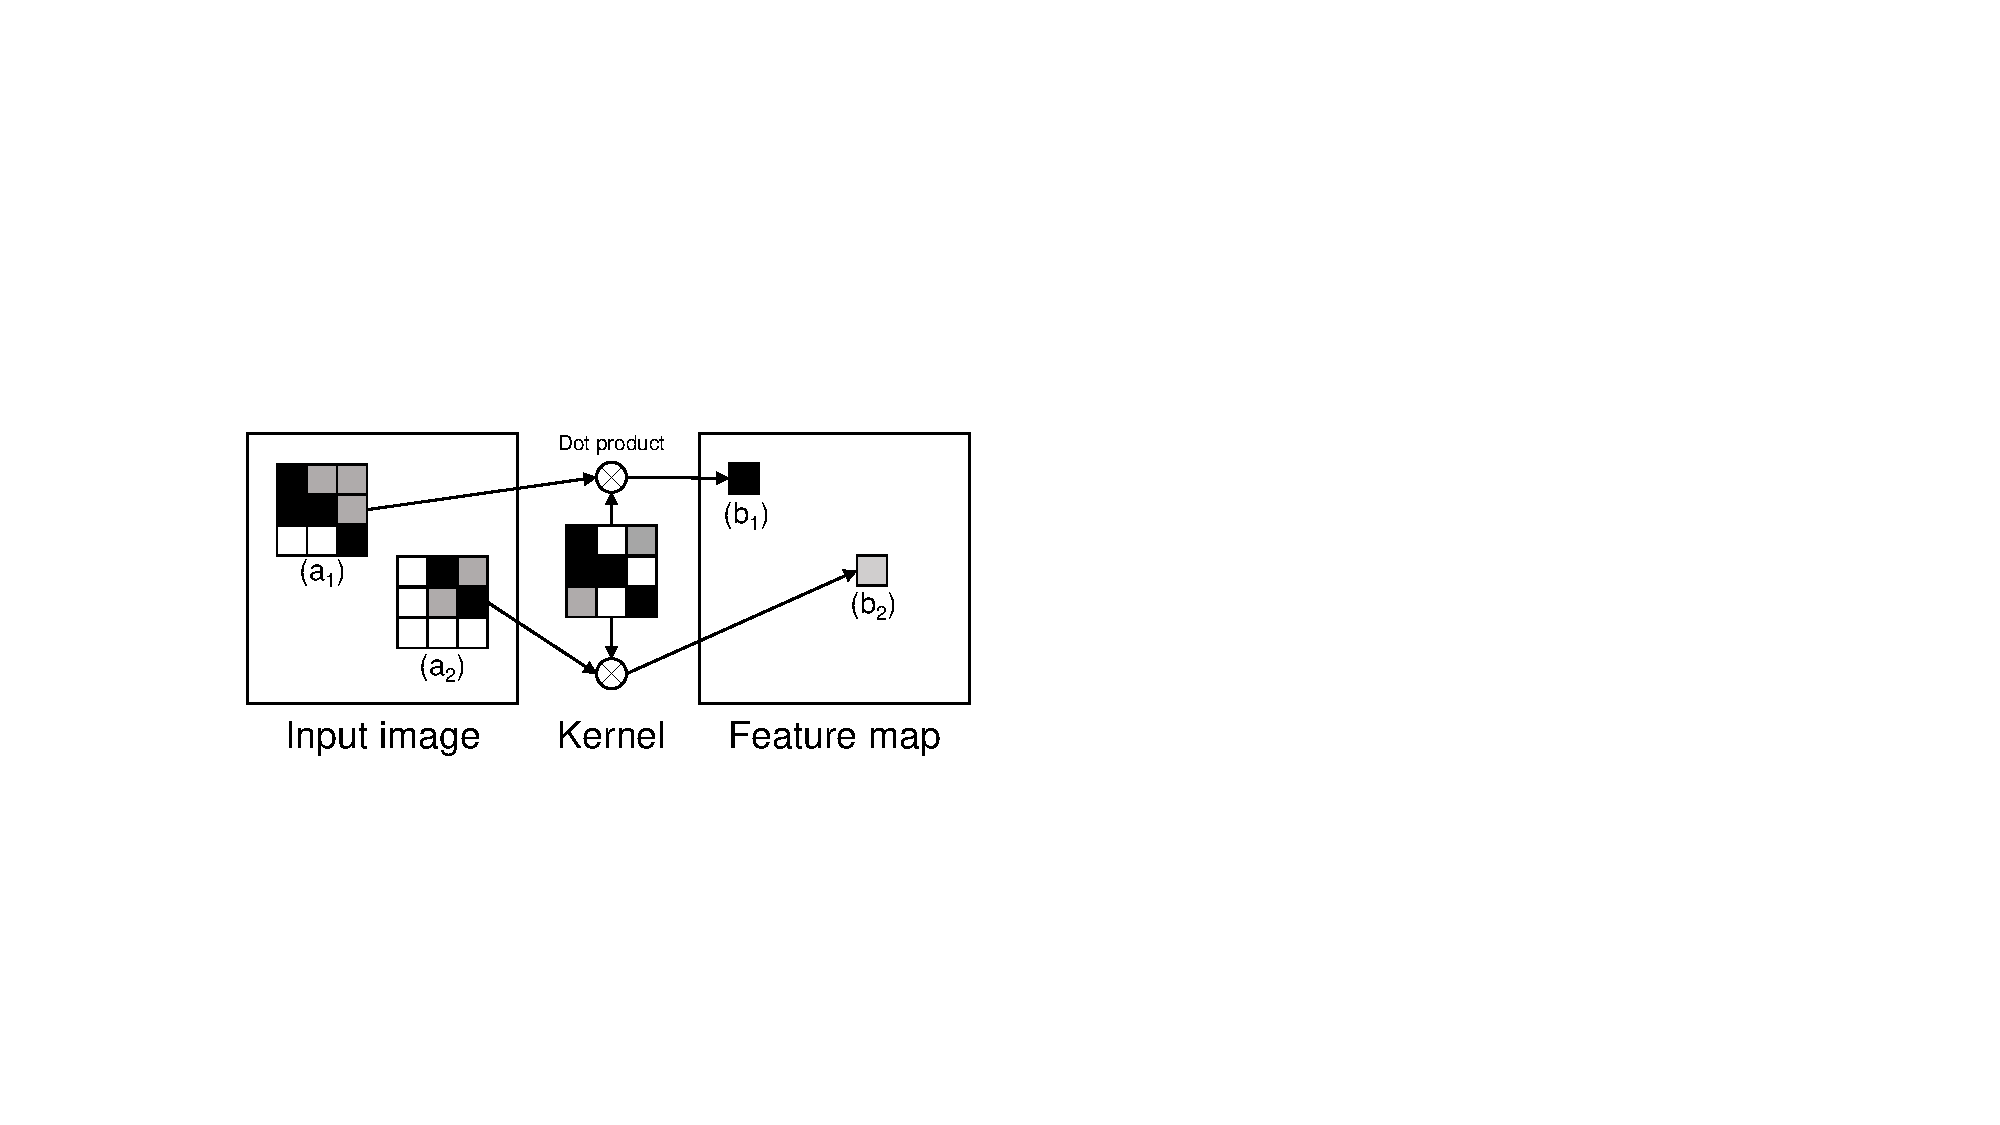
\includegraphics[width=0.7\linewidth]{./figures/feature-map}
  \caption{An example of typical 2D convolutions. }
  \label{fig_conv}
\end{figure}

Such a 2D discrete convolution is widely used in image processing and sometimes called an \textit{image convolution}. An image, $D[h][w]$ in Equation~\ref{2d-conv}, is treated as a function of 2D pixel coordinates in an image convolution. $F[h][w]$ in Equation~\ref{2d-conv} is called a filter or a kernel. The result of the 2D convolution in Equation~\ref{2d-conv} generate a feature map as shown in Figure~\ref{fig_conv}. The size of a filter ($R \times S$) is typically much smaller than the size of the input image ($H \times W$). For a given filter in Figure~\ref{fig_conv}, input image regions (\textit{e.g.}, $a_1$ and $a_2$) with the same size and dimension as the kernel are pointwisely multiplicated with the kernel. A \textit{feature} map consists of all the results (\textit{e.g.}, $b_1$ and $b_2$) of such multiplication. A high value of the result implies that the corresponding region in the input image has a high degree of similarity to the kernel. 

\begin{figure}[htbp]
  \centering
  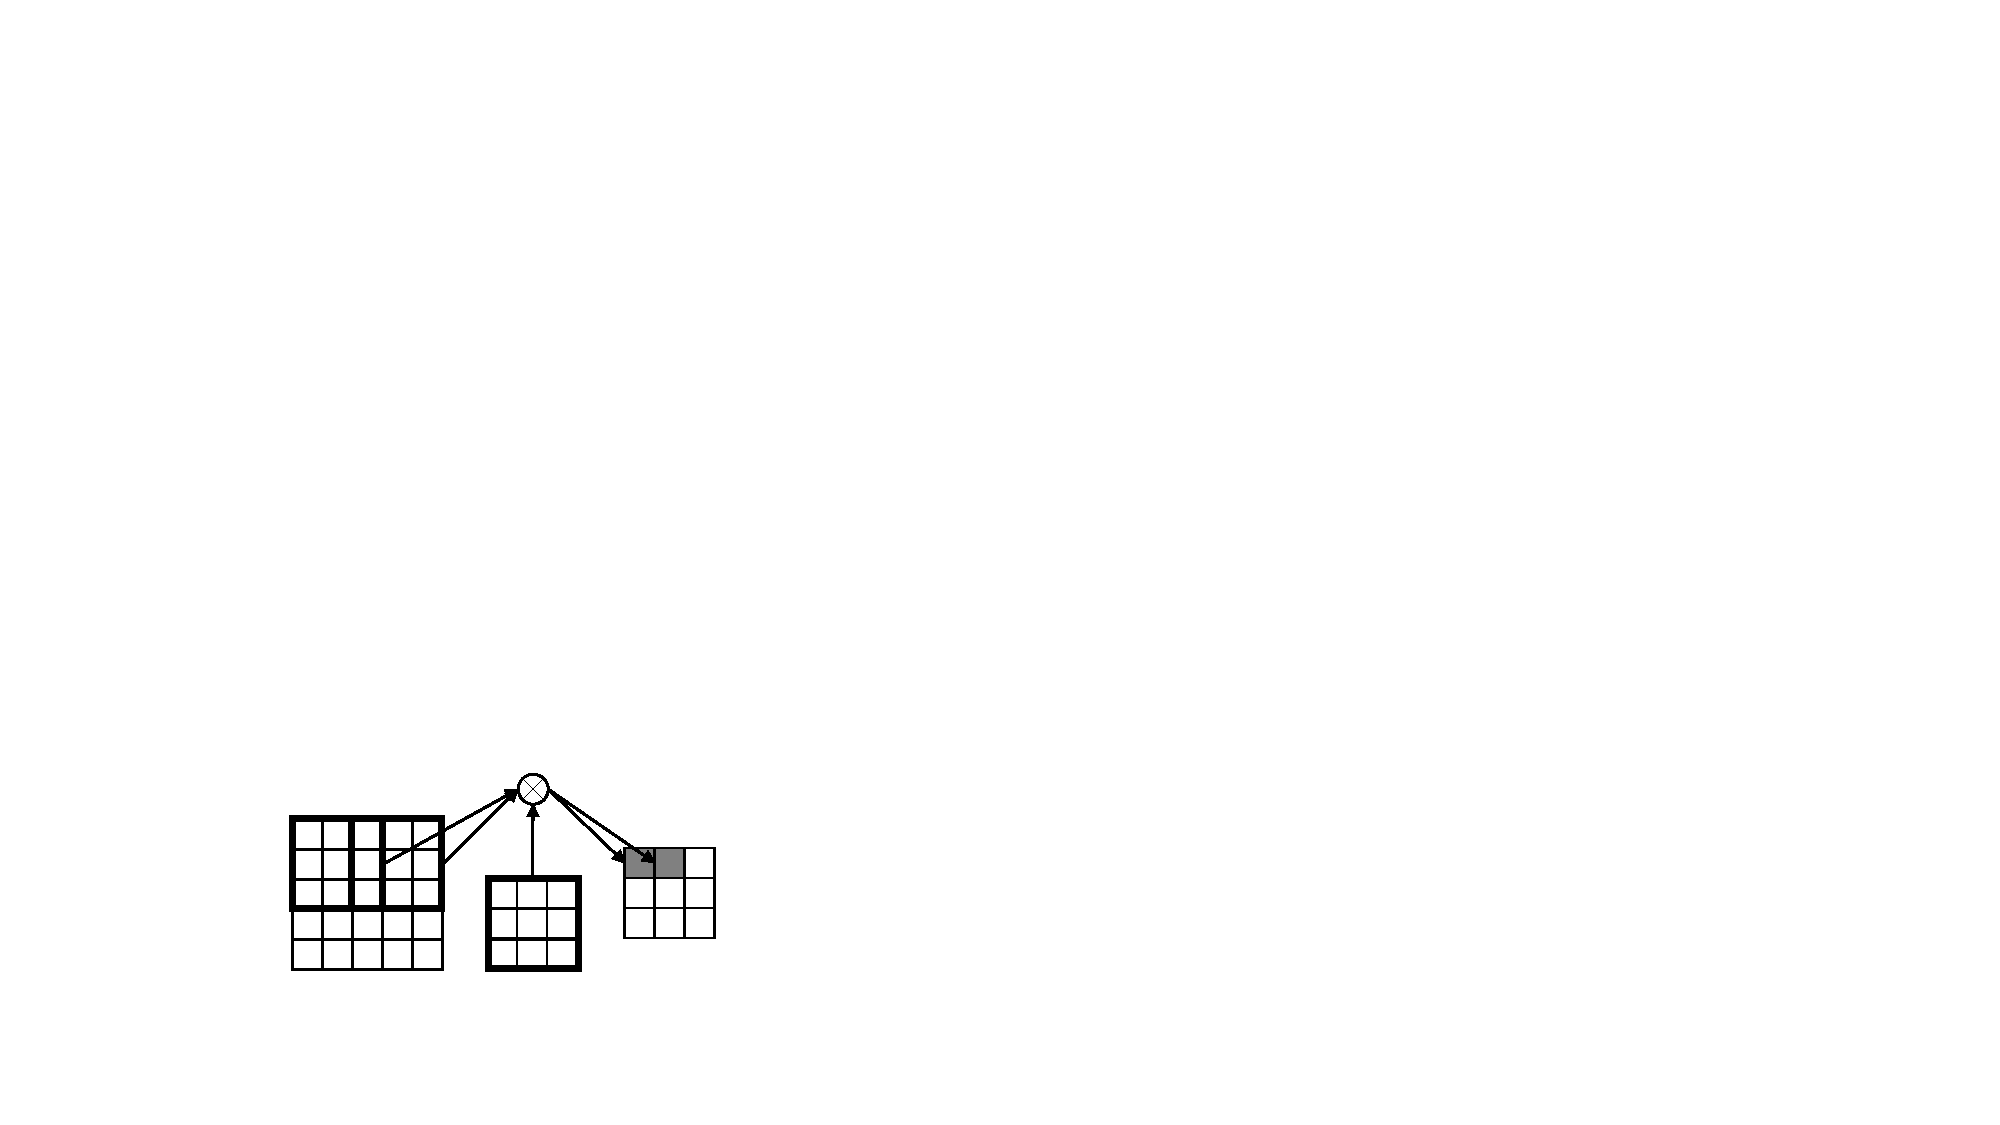
\includegraphics[width=0.5\linewidth]{./figures/stride}
  \caption{Convolution with a stride of two. }
  \label{fig_stride}
\end{figure}

\begin{figure}[htbp]
  \centering
  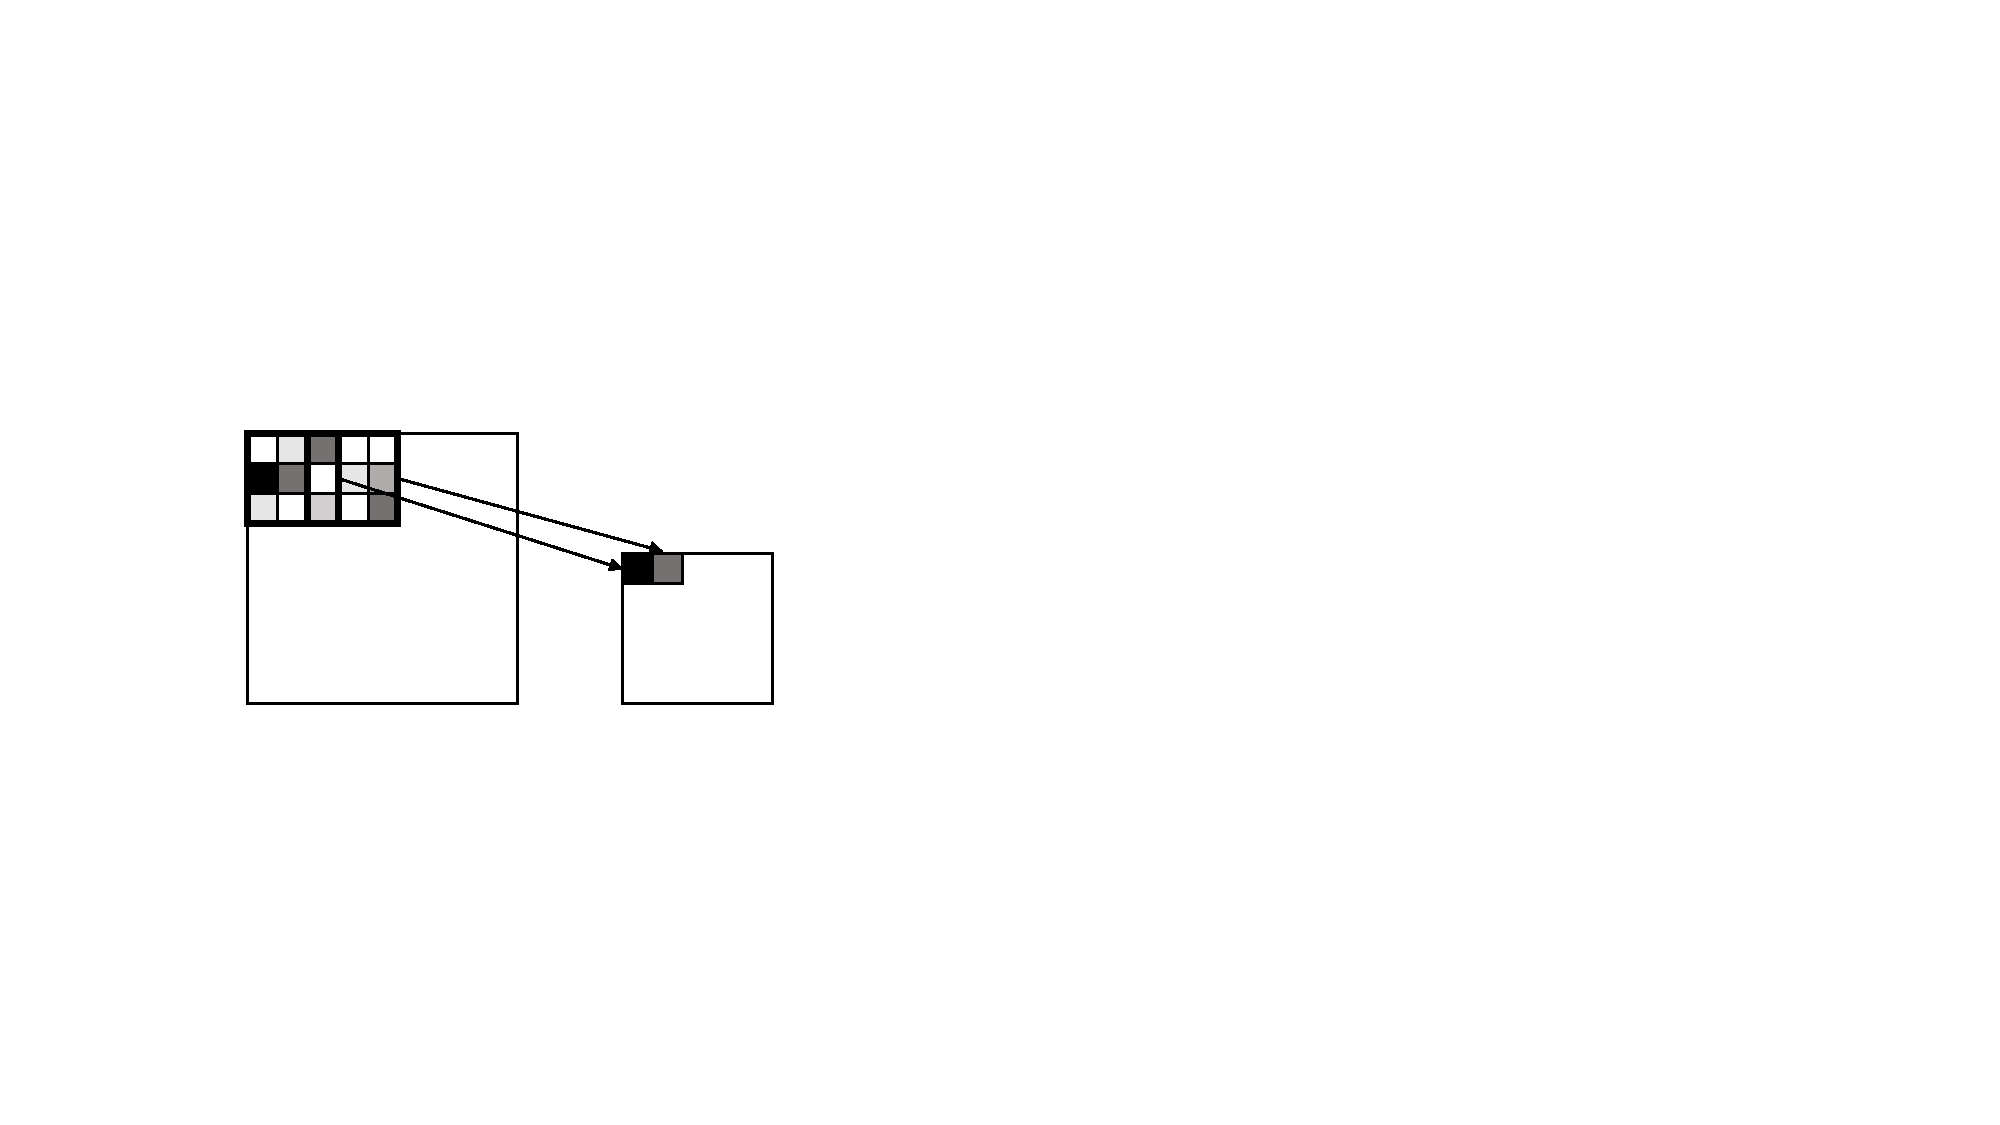
\includegraphics[width=0.5\linewidth]{./figures/pooling}
  \caption{$3 \times 3$ max pooling with a stride of two. }
  \label{fig_pooling}
\end{figure}

Since the convolution operation contains a large amount of computation, there are many techniques introduced to reduce the amount computation. A representative technique is applying the 2D convolution to the input image with a stride as shown in Figure~\ref{fig_stride}. A strided convolution does down-sampling the output of convolution by sampling only every $s$ pixels in each direction of the input image, where $s$ is the value of the stride. Thus, the size of the resulting feature map is smaller than that of the input image. 

Another techinique is \textit{pooling}. Pooling also performs down-sampling and reduces the amount of computation. It identifies a representative pixel for a pixel region to reduce the size of the input. For example, Figure~\ref{fig_pooling} shows $3 \times 3$ \textit{max pooling} with a stride of two. It divides the input in $3 \times 3$-pixel regions with a stride of two. For each region, it selects a pixel that has the maximum value in the region as the representative of the region. 

\subsection{Convolutional Neural Networks}
\label{sec:CNN}
A convolutional neural network (CNN) is an artificial neural network using convolutional filters to extract features from its input. In a CNN, a layer that performs 2D convolutions is called a \textit{convolutional layer}. It typically consists of $N (1 \geq 1)$ filters (\textit{i.e.}, kernels). Since a filter extracts a feature from the input image, a convolution layer estract multiple features from an input image resulting in $N$ feature maps, each of which is also called a \textit{channel}. The training stage of the CNN makes the CNN learn a filter for each of the features.

\begin{figure}[htbp]
  \centering
  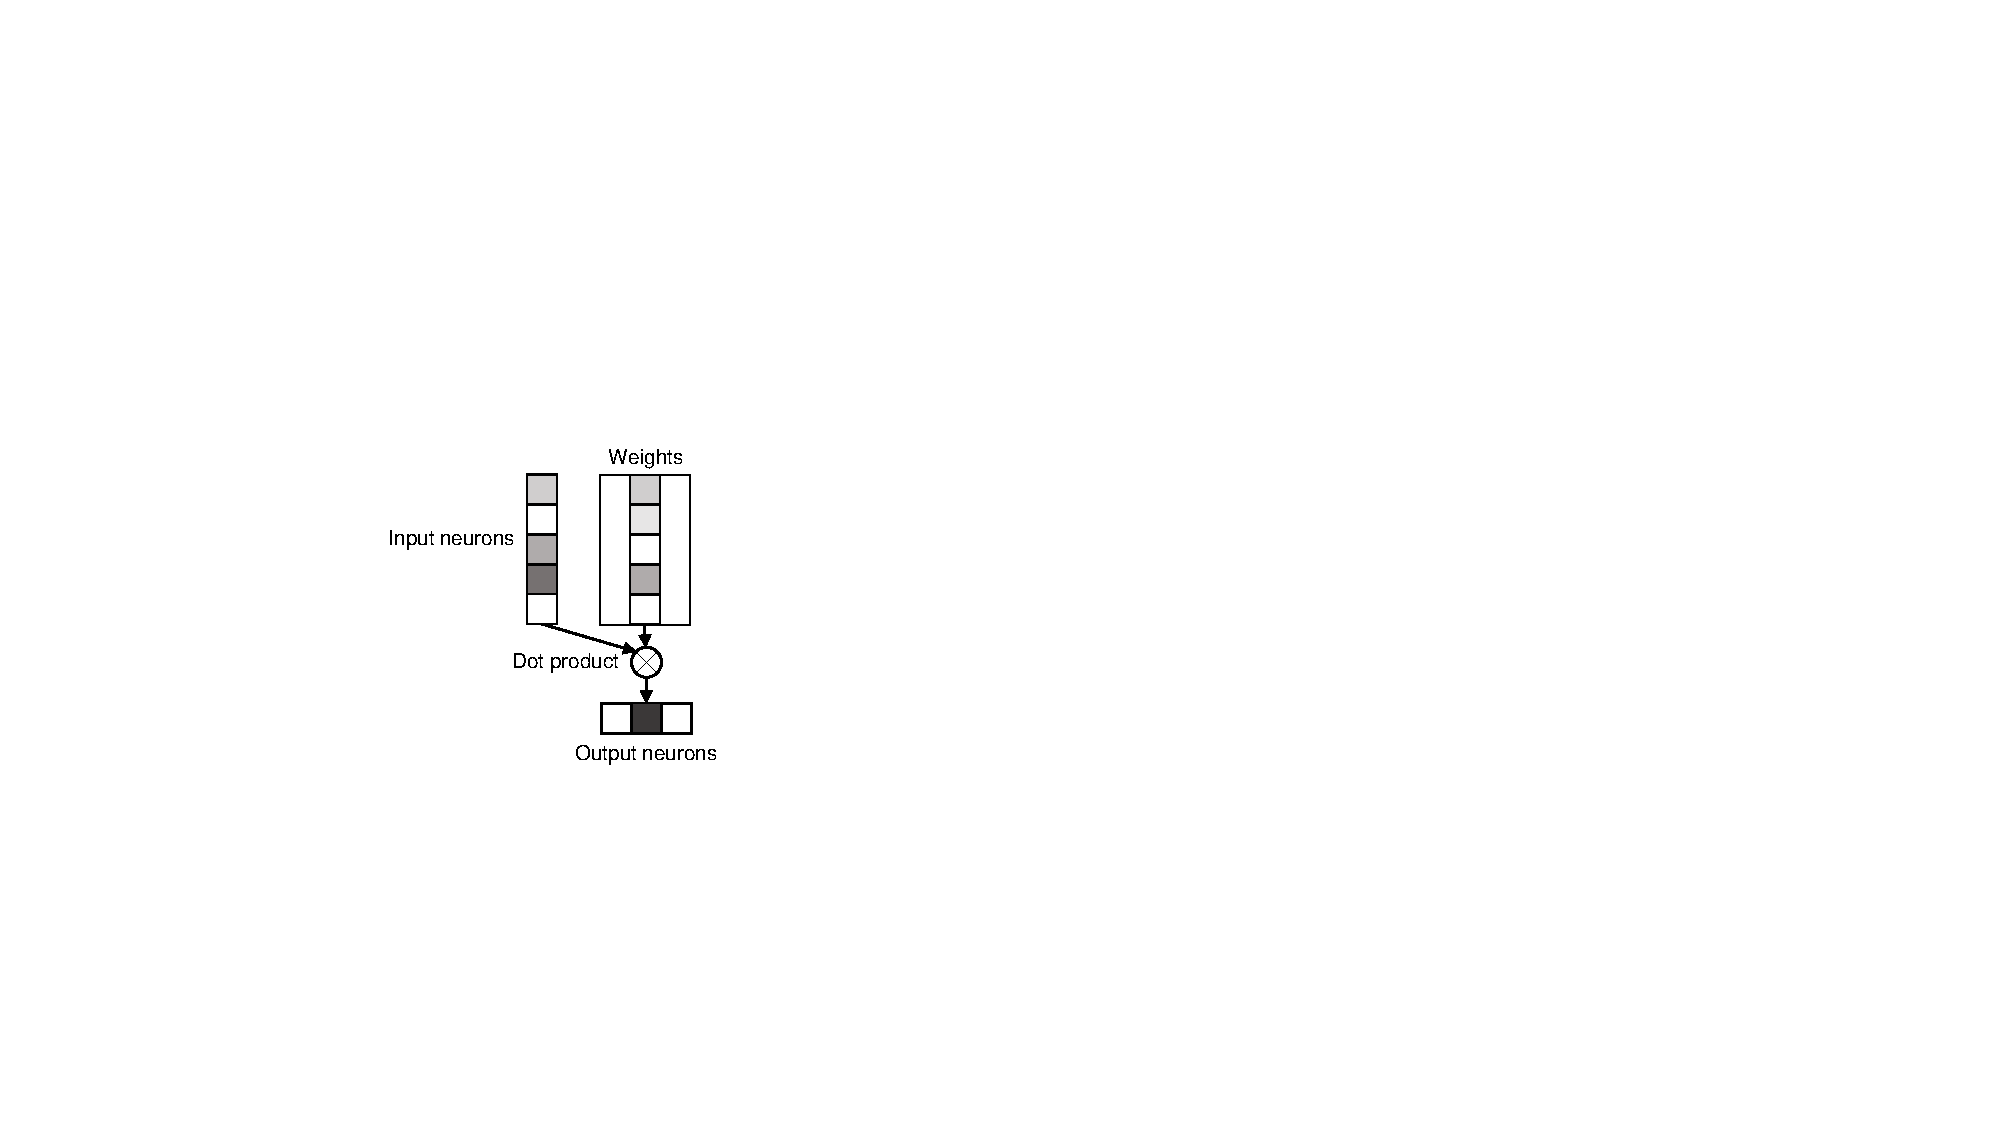
\includegraphics[width=0.5\linewidth]{./figures/fully}
  \caption{Computation in the fully connected layer. }
  \label{fig_fully}
\end{figure}

A \textit{fully connected layer} in a CNN combines the results of convolution. As shown in Figure~\ref{fig_fully}, it consists of input neurons, output neurons, and weights that represent the relationship between the input and output. It performs matrix (the weights) and vector (the input) multiplication and generates the output.

\begin{figure*}[htbp]
  \centering
  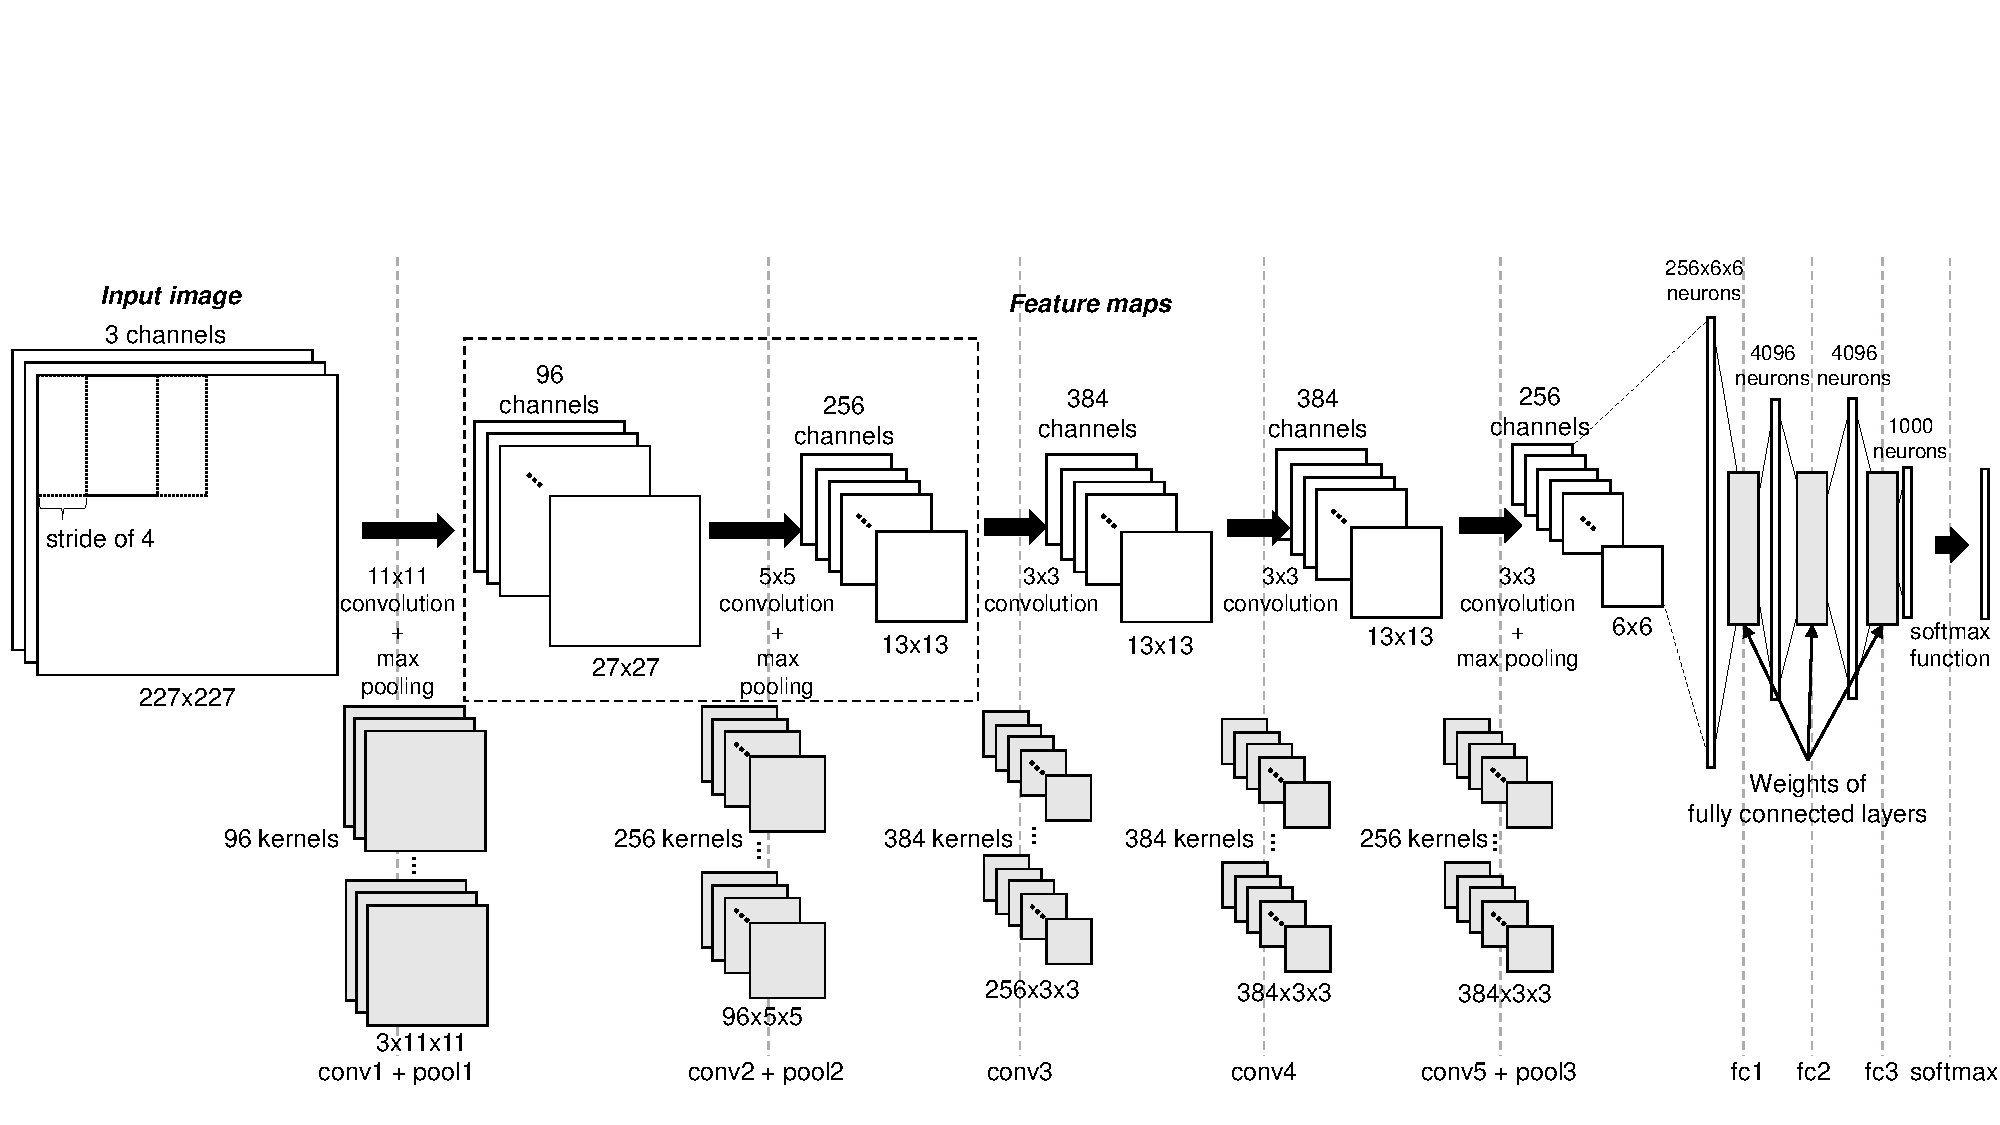
\includegraphics[width=\linewidth]{./figures/Alex}
  \caption{The organization of AlexNet.}
  \label{fig_Alex}
\end{figure*}

\begin{table}[htbp]
\centering
\caption{Configuration of AlexNet}
\label{alex_model}
\begin{scriptsize}
\begin{tabular}{l|l|l|l|l}
\hline
\begin{tabular}[c]{@{}l@{}}Layer\\name\end{tabular}    & 
 \begin{tabular}[c]{@{}l@{}}Kernel size\\ (pooling size) \\ / stride\end{tabular} 
 & Output size     & 
 \begin{tabular}[c]{@{}l@{}}Number of\\ parameters\end{tabular} & 
 \begin{tabular}[c]{@{}l@{}}Number of\\ FP \\operations\end{tabular} \\
\hline
conv1         & 11 x 11 / 4   & 96 x 55 x 55    & 35K        & 55G  \\
pool1         & 3 x 3 / 2     & 96 x 27 x 27    &           &      \\
conv2         & 5 x 5 / 1    & 256 x 27 x 27    & 614K   & 227G \\
pool2         & 3 x 3 / 2    & 256 x 13 x 13    &        &      \\
conv3         & 3 x 3 / 1    & 384 x 13 x 13    & 885K   & 65G  \\
conv4         & 3 x 3 / 1    & 384 x 13 x 13    & 1.3M   & 98G  \\
conv5         & 3 x 3 / 1    & 256 x 13 x 13    & 885K   & 65G  \\
pool3         & 3 x 3 / 2    & 256 x 6 x 6      &        &      \\
fc6           &              & 4096             & 37M    & 74M  \\
fc7           &              & 4096             & 16M    & 32M  \\
fc8           &              & 1000             & 4M     & 8M   \\
softmax       &              & 1000             &        &      \\ 
\hline 
\end{tabular}
\end{scriptsize}
\end{table}

{\bf AlexNet}. Figure~\ref{fig_Alex} shows a representative CNN, AlexNet\cite{krizhevsky2012imagenet}. It is one of the earliest successful DNNs that perform image recognition tasks on the ImageNet dataset\cite{DBLP:journals/corr/RussakovskyDSKSMHKKBBF14}. It uses five convolution layers (conv1, conv2, conv3, conv4, aand conv5) and three max pooling layers (pool1, pool2, and pool3) to extract features. In addition, there are three fully connected layers (fc1, fc2, and fc3) for image classification. Each layer uses the rectified linear unit (ReLU) for nonlinear neuron activation. 

Grey boxes represent kernels and weights of fully connected layers. The input to the first convoluton layer is the input image. The result of a previous convolution layer becomes the input to the next convolution layer after going through a max-pooling layer if there is any. At the beginning, 96 $3 \times 11 \times 11$ 3D kernels are applied to the RGB channels of the input image. This is equivalent to applying 96 $11 \times 11$ 2D kernels to each input image channel. 

The fully connected layers combine the features extracted by the previous convolution layers and creating a conclusion. The output of the last convolution layer after max pooling becomes the input neurons of the first fully connected layer. For a given image, AlexNet determines which image class it belongs to among 1000 predefined image classes. The last layer, \textit{softmax} layer, normalizes the output values of the last fully connected layer and converts the output to the values of probability. The last fully connected layer and the softmax layer have 1000 output neurons, respectively, each of which corrosponds to one of the image classes. The probability value of each softmax neuron represents the confidence level that the input image belongs to the associated class with the neuron.

\begin{figure}[htbp]
  \centering
  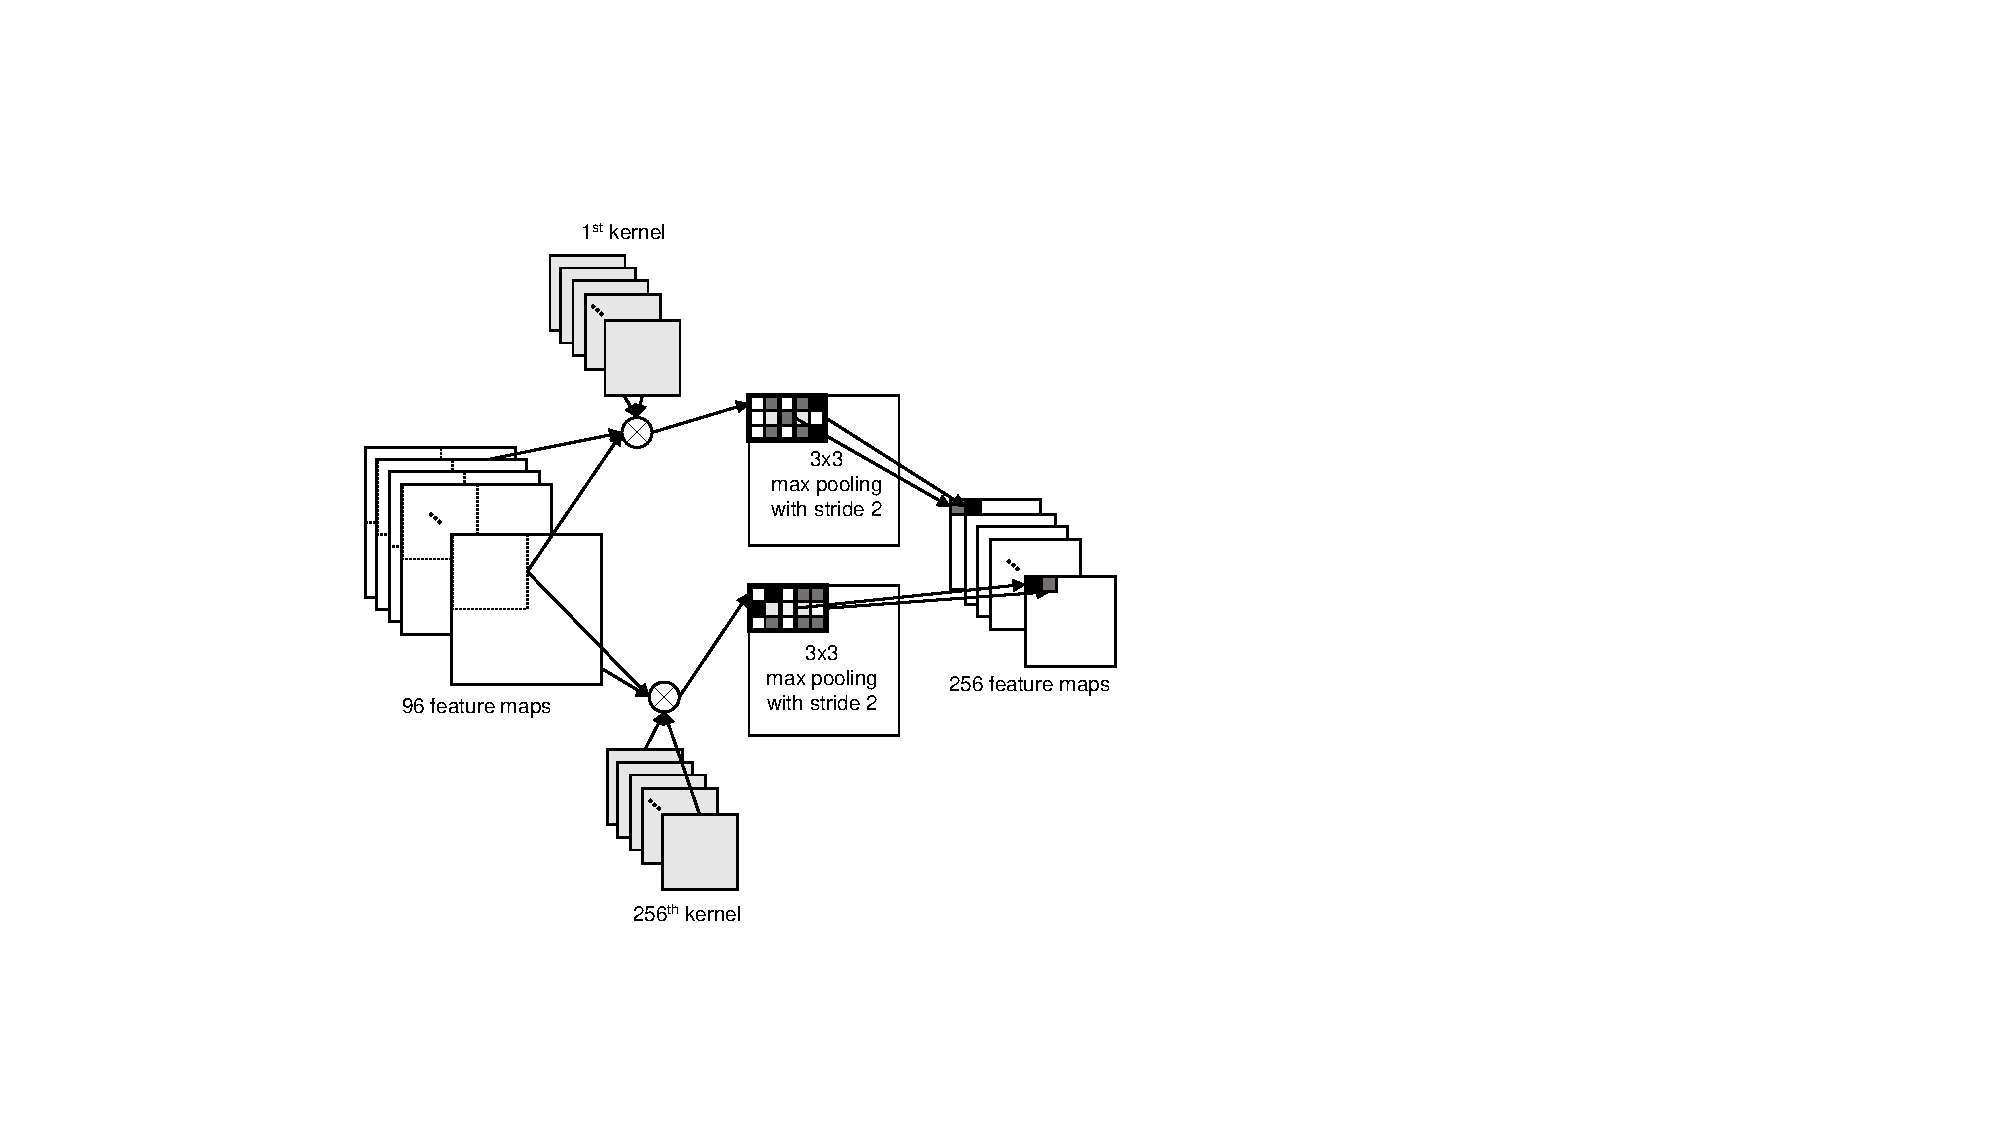
\includegraphics[width=\linewidth]{./figures/convolution}
  \caption{An example of convolution computation in AlexNet.}
  \label{fig_convolution}
\end{figure}

The dotted box in Figure~\ref{fig_Alex} is detailed in Figure~\ref{fig_convolution}. The 96 feature maps produced by the previous layer are convolved by 256 $5 \times 5 \times 96$ 3D kernels and go through $3 \times 3$ max pooling with a stride of two resulting in 256 new feature maps. Since there are 96 inputs, applying a $5 \times 5$ 2D kernel to each of the 96 inputs is equivalent to applying a $5 \times 5 \times 96$ 3D kernel to the 96 inputs. The detailed configuration of the AlexNet model in this study is presented in Table~\ref{alex_model}.

AlexNet has been frequently used for benchmarking deep learning libraries because it is equiped with most of the state-of-the-art DNN components, such as convolution, max-pooling, and dropout\cite{convnet-benchmarks}. The original AlexNet model includes a local response normalization (LRN) layer, but we exclude it in this study because LRN is very rarely used in current convolutional neural networks. 

{\bf Training.} Training a CNN is a supervised learning process using training images and correct class labels that are associated with the training images. It has two stages: \textit{forward computation} and \textit{backward computation}. For a given training image, the forward computation stage goes through the CNN layers from the first to the last and obtains the output from the last layer. For example, AlexNet determines the class to which the training input image belongs. After computing the difference between the output and the correct label, the backward compuation stage obtains the values that need to be added to the parameters (\textit{e.g.}, weights) of the last fully connected layer by computing gradients. After updating the parameters in the last layer with the gradients, these values are backward propagated to the previous layers (\textit{i.e.}, \textit{backpropagation} is performed) to adjust their parmeters in the backward computation stage. The gradients are computed in the direction of minimizing the difference between the output and the correct label.

{\bf Batch of inputs}. When a CNN is trained, training inputs (images) are divided in to sets of images, each of which is called a \textit{batch}. A batch is processed by the CNN at a time. This is because the stochastic gradient decent technique (SGD)\cite{onlinesgd} that is typically used to obtain the gradients can be easily parallelized across different images in the same batch. 

{\bf 4D tensor}. Since multiple 2D feature maps are typically processed in a layer at a time, and multiple images in a batch are processed at a time, the feature map data in a CNN can be treated as four-dimensional tensors $<N, C, H, W>$, where $N$, $C$, $H$, and $W$ are the number of images in a batch, the number of channels (\textit{i.e.}, feature maps), the height of a feature map, and the width of a feature map, respectively. Since the 4D tensor data are stored in the order of the dimensions $N$, $C$, $H$, and $W$, they are called $NCHW$ 4D tensors. The computational complexity of convolving a $NCHW$ tensor with $K \times R \times S$ 3D kernel is $O(K \times CRS \times NHW)$.

\begin{figure}[htbp]
  \centering
  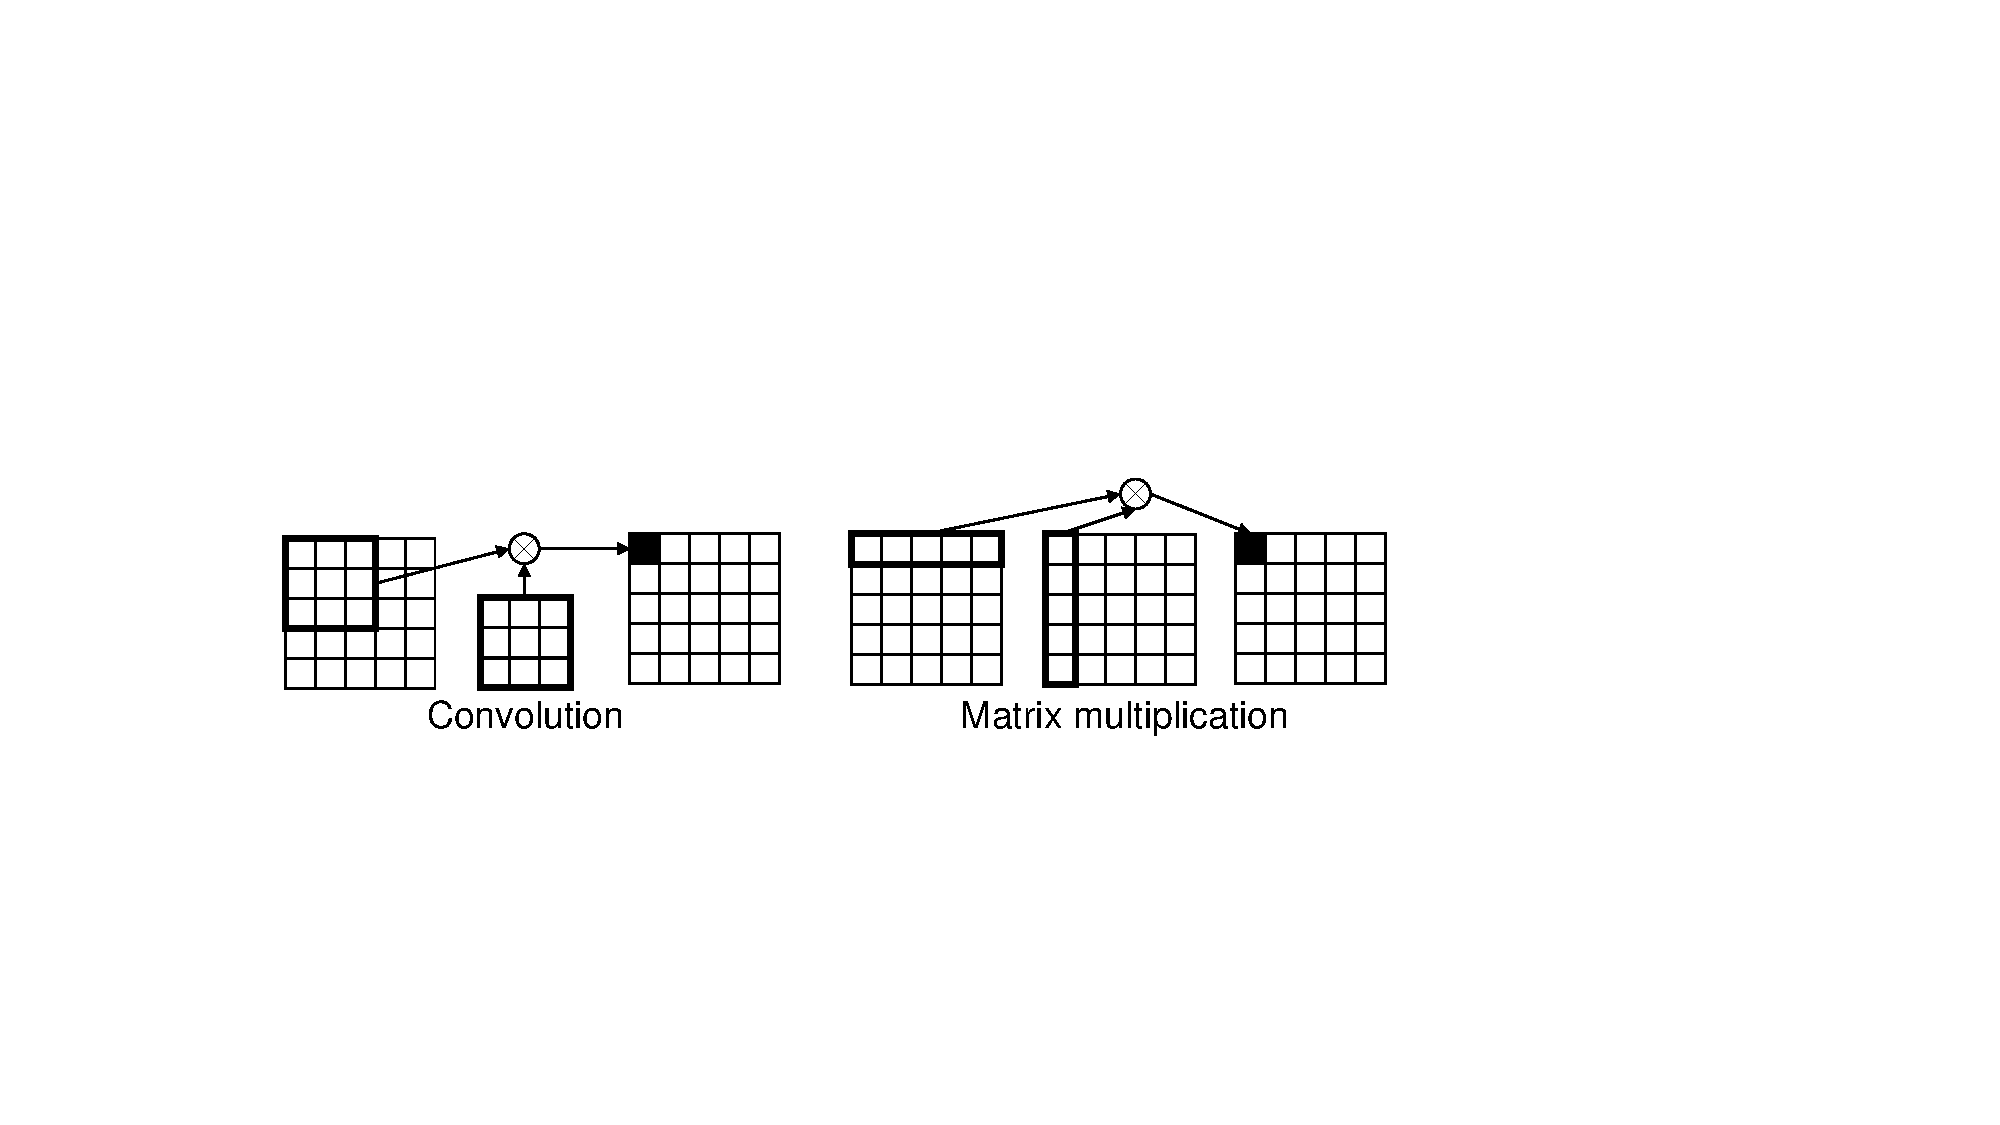
\includegraphics[width=0.5\linewidth]{./figures/direct}
  \caption{Direct convolution computation vs. matrix multiplication.}
  \label{fig_direct}
\end{figure}

\subsection{Convolution Algorithms}
\label{sec:algorithms}
{\bf Direct convolution}. Since the efficiency of convolution computation is important to CNNs, several methods have been developed to efficiently implement the convolution operation on a GPU. Directly computing the convolution (we call it \textit{direct convolution} in this paper) using Equation~\ref{2d-conv} is the most straightforward way to peform convolution. However, it needs a lot of specialized GPU kernels to optimize it for various input dimensions and corner cases. Cuda-convnet\cite{cuda-convnet} is a widely used direct convolution library. Figure~\ref{fig_direct} compares matrix multiplication and direct convolution computation.

\begin{figure}[htbp]
  \centering
  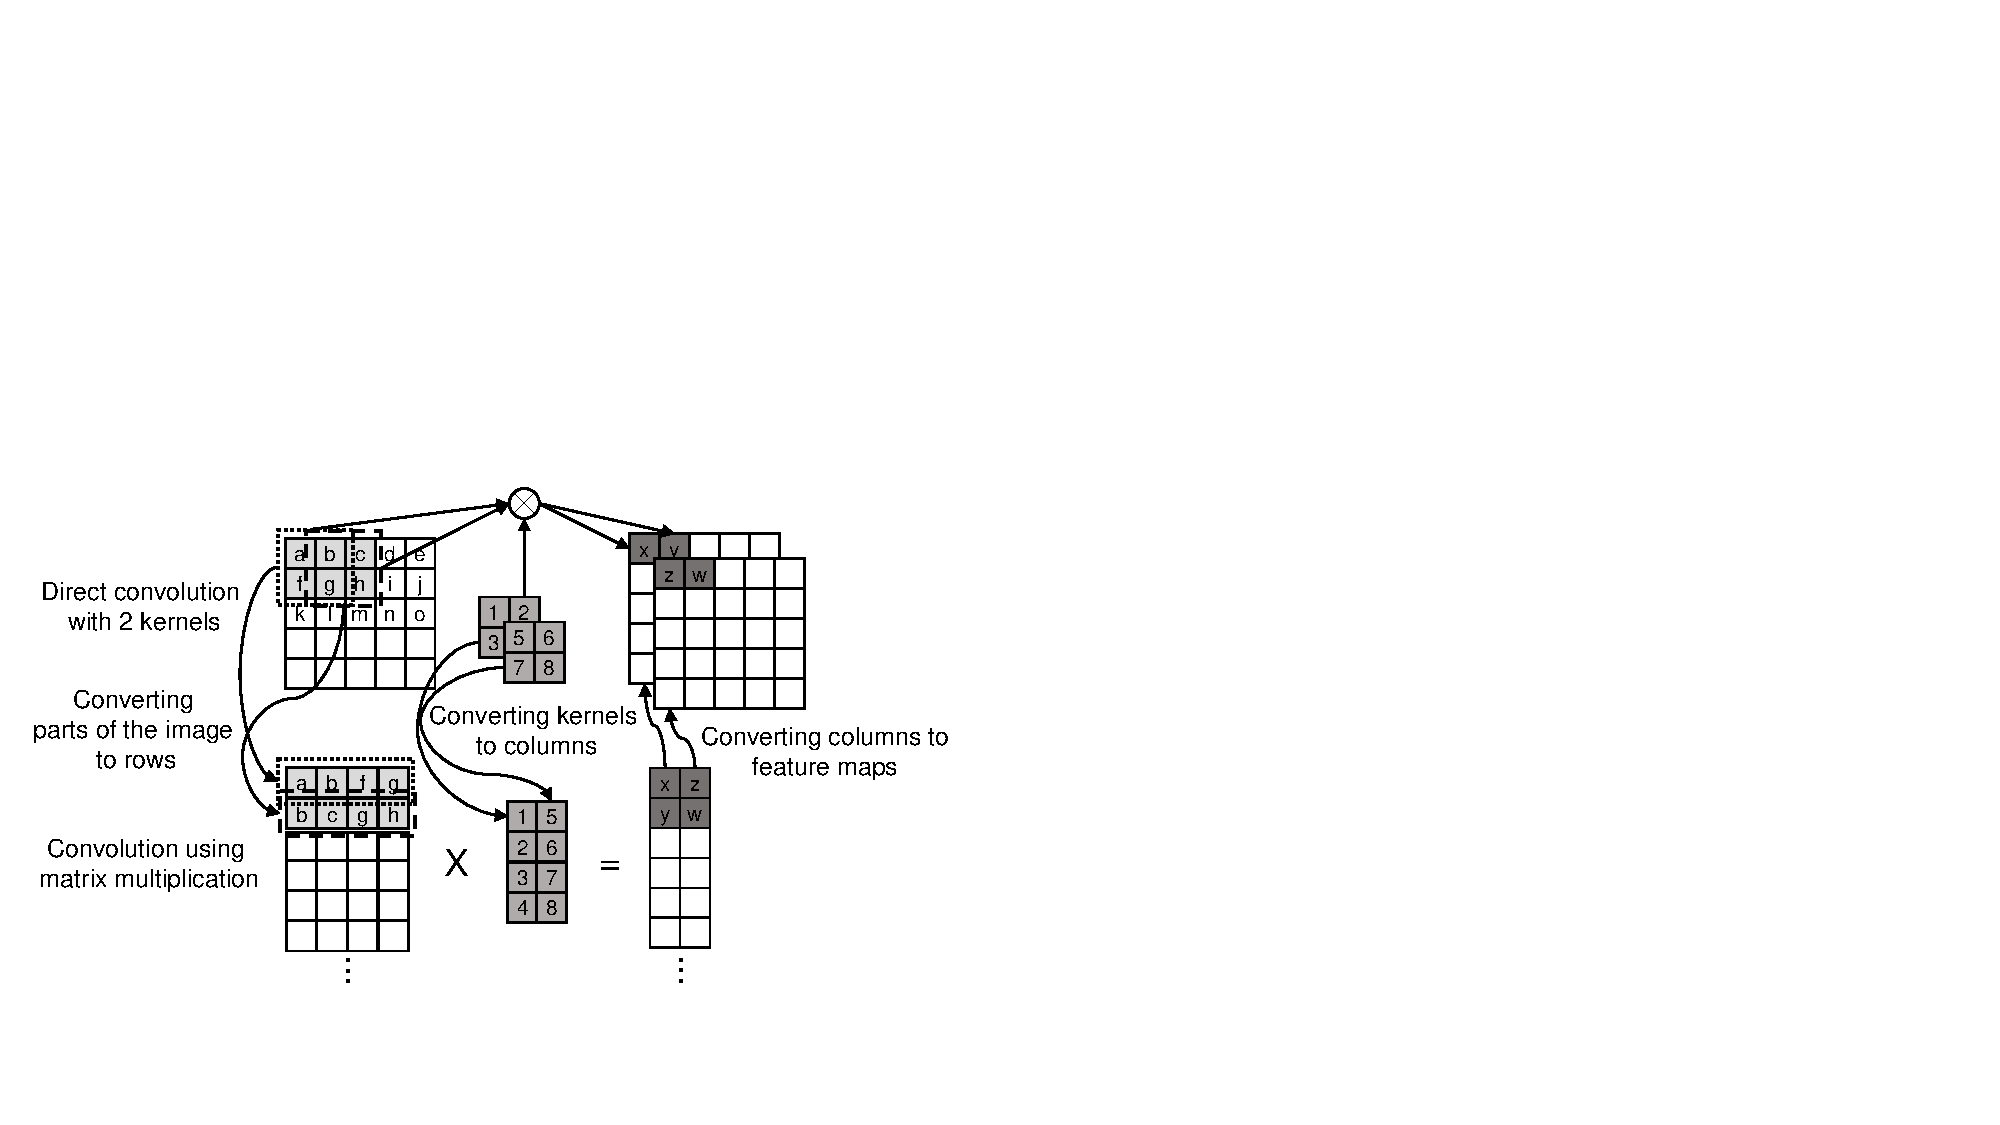
\includegraphics[width=\linewidth]{./figures/matmul}
  \caption{Convolution using matrix multiplication.}
  \label{fig_matmul}
\end{figure}

{\bf Using matrix multiplication}. CuDNN\cite{cudnn}, a DNN library from NVIDIA, treats the convolution as matrix multiplication (\textit{e.g.}, GEMM\cite{cublas}). Figure~\ref{fig_matmul} illustrates an example. It convolves a $5 \times 5$ image with two $2 \times 2$ kernels and obtains two $5 \times 5$ feature maps. When the input image has multiple channels, a row in the imput matrix contiguously contains pixels from the multiple channels. When the number of input channels, the size of a kernel, the number of kernels, and the input image size are $C$, $R \times S$, $K$, and $H \times W$, respectively, the sizes of the input matrix and the kernel matrices become $CRS \times WH$ and $K \times CRS$, respectively. Since the complexity of the matrix multiplication is $O(K \times CRS \times WH)$, when the number of images in a batch is $N$, the complexity becomes $O(K \times CRS \times NWH)$. 

Interestingly, the computational complexity of this matrix multiplicaiton method is the same as that of the direct convolution computation. However, the matrix mutiplication can be parallelized using highly efficient BLAS libraries\cite{cublas}. Morever, it enables exploiting the GPU local memory that has a low latency and high bandwidth. CuDNN performs the multiplication by applying tiling in the GPU local memory to the matrices. This method scales well with a small batch size and can be used on all types of convolution layers. 

{\bf Using FFT}. FFT convolution uses a fast Fourier transform algorithm to reduce computational complexity\cite{fftconv}. Its complexity is $O(K \times CWW \times \log W)$ that does not depend on the size of the kernel. However, the FFT convolution requires more memory space because filters need to be padded to the dimension of inputs. Another restriction of the FFT convolution is that it can be applied to only convolutions with the stride of one.

{\bf Using the Winograd algorithm}. Winograd convolution is based on GEMM\cite{cublas}. It reduces the algorithmic complexity using Winograd's minimal filtering algorithm\cite{winograd}. It is similar to the well known Strassen's algorithm\cite{winograd1980arithmetic} for matrix multiplication. It reduces matrix multiplication operations significantly when the kernel size is fixed. Thus, a different kernel size requires a different minimal filtering algorithm. The minimal filtering algorithm for 4x3 tiled matrix can reduce 12 multiplication to 6. Nesting the minimal filtering algorithm twice would reduce algorithm complexity by 4\cite{winograd}. CuDNN 5.1 supports Winograd convolution only for the filter sizes of $3 \times 3$ and $5 \times 5$.

\subsection{Multi-GPU Support}
\label{sec:multiGPU-parallelism}
Multi-gpu support of deep neural networks can be implemented by exploiting \textit{data parallelism} or \textit{model parallelism}\cite{NIPS2012_4687}. Exploiting data parallelism means that input images in a batch are divided and distributed accross multiple GPUs and processed by all the GPUs. All the GPUs have the entire network parameters. In the backward computation stage, each GPU computes its own gradients for the inputs assigned to it, then a single device (a CPU or a GPU) combines the gradients computed by all the GPUs and performs the SGD. Network parameters are updated with the result of the SGD, and they are distributed across the GPUs again. This process implies that the communication cost depends on the number of network parameters. Since AlexNet has 62M parameters and their size is 250MB, each iteration (\textit{i.e.}, a batch) needs to transfer approximately 250MB of data per GPU. Quantization methods that approximate the value of a floating-point number with an integer can reduce the amount of data transfer\cite{deepcompress}. CNTK provides 1-bit SGD method that quantizes 32-bit gradient values in to a single bit with some accuracy loss\cite{1-bit-stochastic-gradient-descent-and-application-to-data-parallel-distributed-training-of-speech-dnns}.

On the other hand, the model parallelism makes users to divide and distribute the network itself across GPUs. Since parameter updates can be done on each GPU using model parallelims, only a small amount of data is communicated between GPUs. A convolution layer using carefully designed model parallelism typically outperforms data parallelism\cite{DBLP:journals/corr/YadanATR13}.

Tensorflow and Torch support both data parallelism and model parallelism. While Caffe and CNTK supports only data parallelism, multi gpu support of Theano is still in experimental stage. Thus, for fairness, we compare only the efficiency of data parallelism between Caffe, TensorFlow, Torch and CNTK for multiple GPUs. 

\subsection{Related Work}
Since it has been only a few years since deep learning frameworks were introduced to public, not that many previous studies compare their performance. Recently, some comparative studies for the deep learning frameworks are performed by Bahrampour \textit{et al.}\cite{DBLP:journals/corr/BahrampourRSS15} and Shi \textit{et al.}\cite{DBLP:journals/corr/ShiWXC16}. However, they show only the entire execution times of various DNN models built by the deep learning frameworks. They do not identify performance bottlenecks and reasons for differences in performance. Moreover, they use cuDNN version R4 that does not support the Winograd convolution algorithm.

A benchmark result for some CNN frameworks is publicly available on Github\cite{convnet-benchmarks}. It reports forward and backward computation times of a CNN model. The latest result was produced with cuDNN version R4, while the most recent cuDNN version is R5.1. This paper uses cuDNN version R5 and R5.1.
